%=======================+=========================
%================  Controls  ================
%=================================================

\section[Slow controls]{Slow controls \label{sec:controls}}
\GX{} must monitor 
and control tens of thousands of different variables that define the state of the experimental hardware. Different variable values need to be acquired, displayed, archived, and used as inputs to control loops continually with a high degree of reliability. For \gx, approximately 90,000 variables are archived, and many more are monitored.

\subsection{Architecture \label{sec:controlsarchitechture}}
The \gx{} slow control system consists of three layers. The first layer consists of the remote units such as high voltage or low voltage power chassis, magnet power supplies, temperature controller, LabView applications, and PLC-based applications, which directly interact with the hardware and contain almost all the control loops. The second layer is the Supervisory Control and Data Acquisition (SCADA) layer, which is implemented via approximately 140 EPICS Input/Output Controllers (IOC's). This layer provides the interface between low level applications and higher level applications via the EPICS ChannelAccess protocol. The highest level, referred as the Experiment Control System (ECS), contains applications such as Human-Machine Interfaces, the alarm system, and data archiving system. This structure allows for relatively simple and seamless addition and integration of new components into the overall controls system.    

\subsection{Remote Units \label{sec:controlsinterface}}
\gx{} uses a variety of commercial units to provide control over the hardware used in the experiment. For instance, most detector high voltages are provided by the CAEN SYx527 voltage mainframe,\footnote{https://www.caen.it/subfamilies/mainframes/} while the low and bias voltages are provided by boards residing in a Wiener MPOD chassis\footnote{http://www.wiener-d.com/sc/power-supplies/mpod--lvhv/mpod-crate.html}. These two power supply types provide most voltages for detector elements with the exception of Tagger Microscope and Forward Calorimeter where custom systems were developed that provide voltage regulation and interact with the EPICS-based layer through higher level interfaces using custom protocols. See Sections.~\ref{sec:TAGM} and \ref{sec:fcal} for more details.  

Various beam line devices need to be moved during beam operations. Stepper motors are used to move motorized stages via Newport XPS universal multi-axis motion controllers\footnote{https://www.newport.com/c/xps-universal-multi-axis-motion-controller.} that allow for execution of complex trajectories involving multiple axes. All stage referencing, motion profile computations, and encoder-based closed-loop control occur within the controller chassis after the basic parameters, such as positions and velocities, are provided by the user via a TCP/IP-based interface to EPICS.   

While installing complex systems, such as a superconducting magnet that requires large numbers of input and output channels and sophisticated logic, custom controls systems were developed for each particular system. For those cases, we used Allen-Bradley CompactLogix and ControlLogix PLC systems\footnote{https://ab.rockwellautomation.com.}. These systems are designed for industrial operations, allow modular design, provide high reliability, and require minimal maintenance. All controls loops are programmed within the PLC application, and are interfaced with EPICS through a TCP/IP-EtherNet/IP-proprietary protocol to allow access by higher level applications to process variables served by the PLC's.  

The cryogenic target and the superconducting solenoid employ National Instruments LabView applications. The target controls use both custom-made and vendor-supplied hardware that include built-in remotely-accessible control systems and an NI CompactRIO\footnote{https://www.ni.com/en-us/shop/compactrio.html} chassis. This chassis communicates with the hardware and serves variables using an internal ChannelAccess server and an EPICS IOC running on the CompactRIO controller, as described in Sec.~\ref{sec:target}. A National Instruments PXI high-performance system\footnote{https://www.ni.com/en-us/shop/pxi.html} is used to collect data from different sensors as described in Sec.~\ref{sec:solenoid}. 

\begin{landscape}
 \begin{figure}[tbp]
\begin{center}
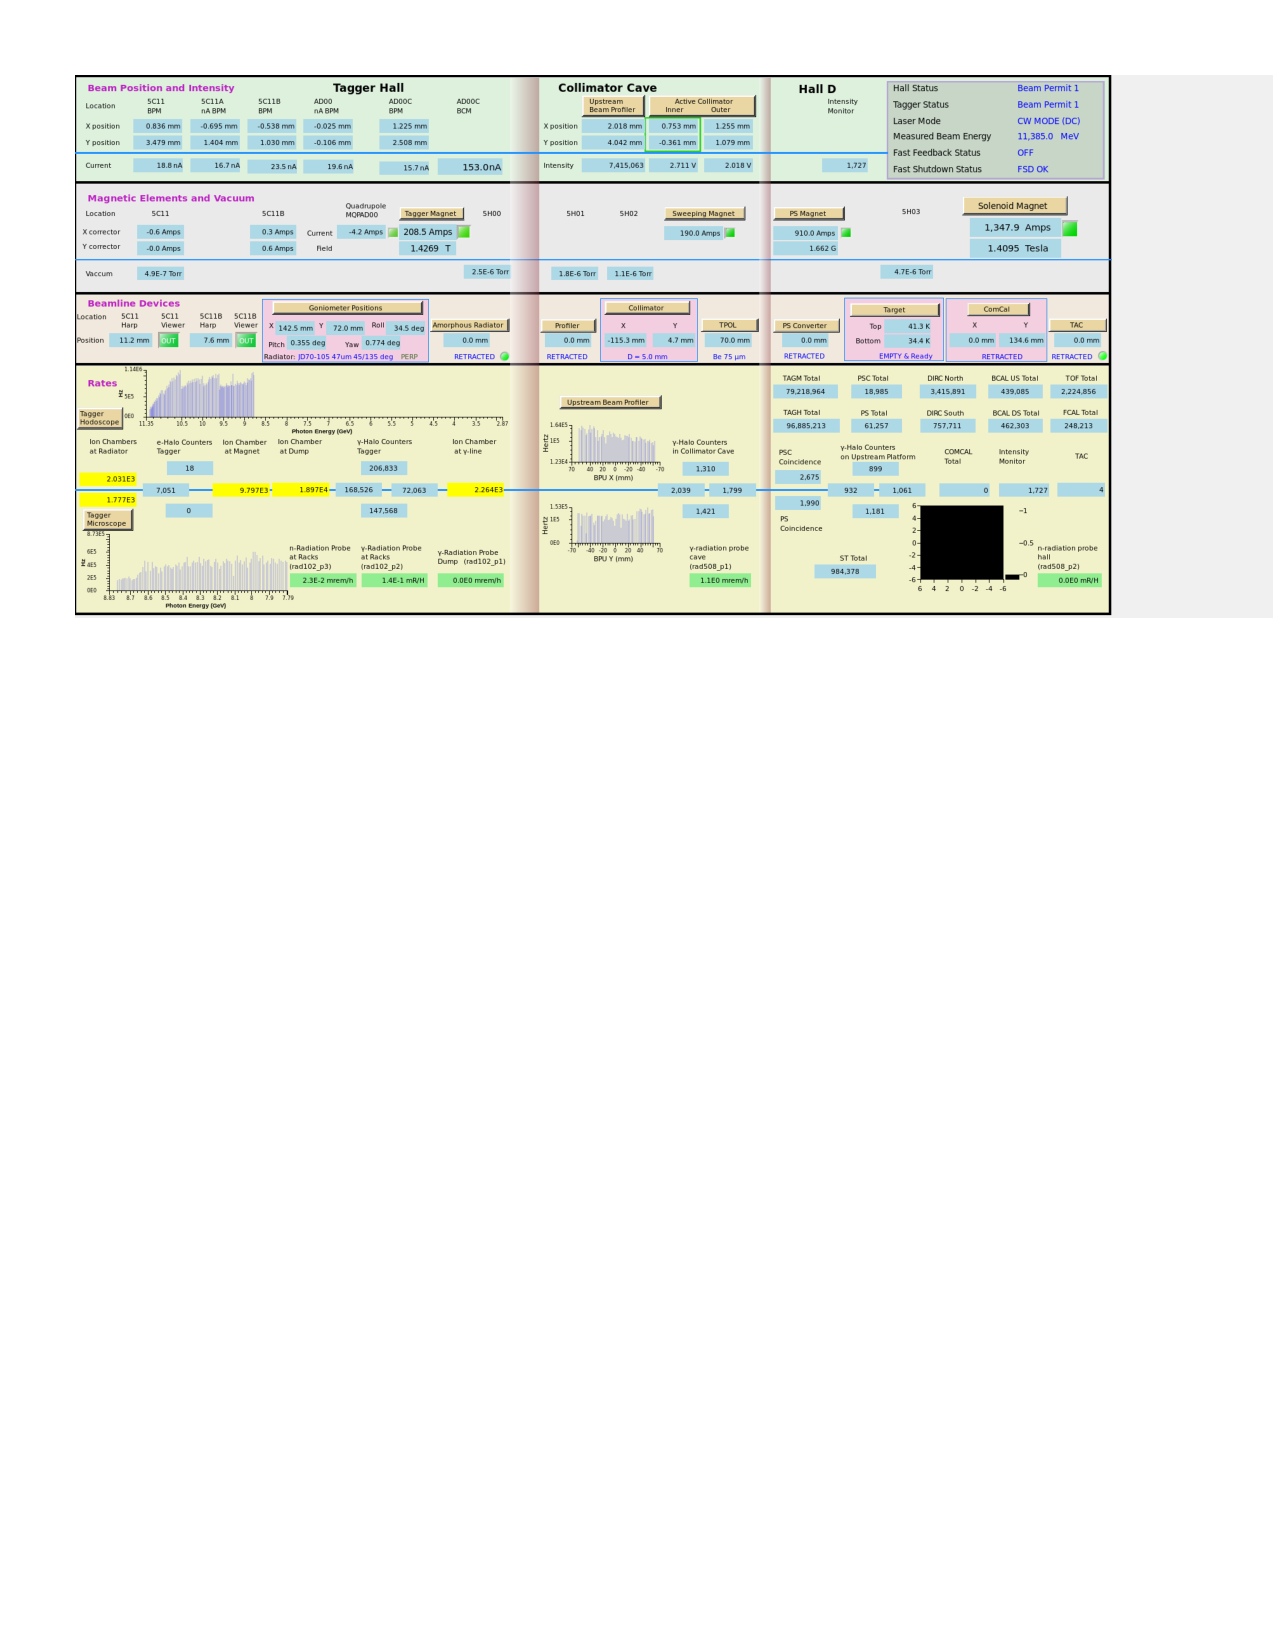
\includegraphics[height=10cm,bb=35 480 535 760,clip=true]{figures/GlueX_CSS_overview.pdf}
%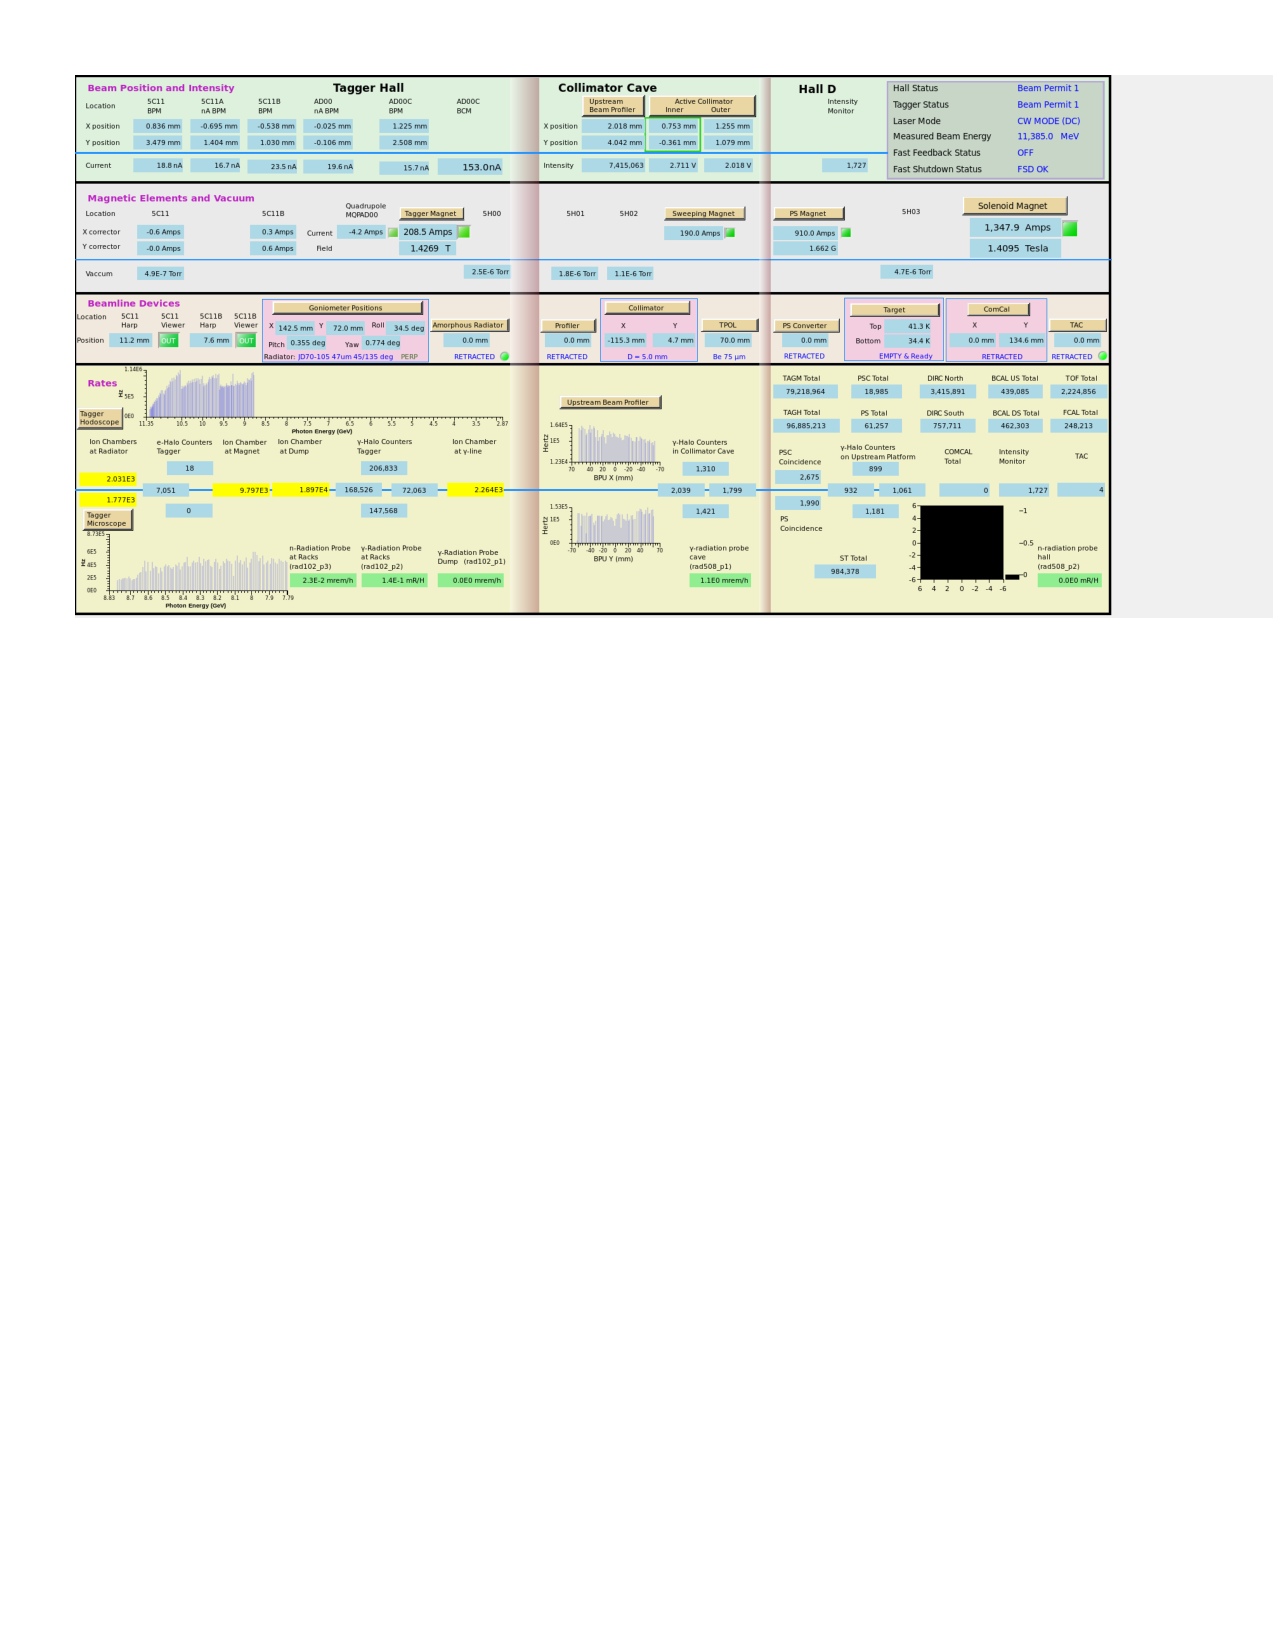
\includegraphics[height=8cm,clip=true]{figures/GlueX_CSS_overview.pdf}
\caption{Top-level graphical interface for the beamline. This screen provides information on beam currents and rates, radiators, magnet status, target condition, background levels, etc.
\label{fig:GlueX_CSS_overview}
}
\end{center}
\end{figure}
\end{landscape}

\subsection{Supervisory Control and Data Acquisition layer \label{sec:archiver}}
The SCADA layer is the middle layer that distributes the process variables allowing the higher level --and sometimes lower level-- applications to use various process variables of the Hall-D control system. This layer is based on EPICS and uses the ChannelAccess protocol to publish the values of the variables over Ethernet. Because the accelerator controls also use EPICS, efficiently exchange the information between the experiment and accelerator operations is achieved. Several dozen software IOC processes running on hosts in the experiment control room collect data from different components of the lowest layer. Each IOCs is configured to communicate using the protocol appropriate for the remote units with which data exchange is needed. For instance, the IOC controlling the voltage for the FDC detector needs to be able to communicate with the Wiener MPOD and CAEN SYx527 voltage chassis. Although the middle layer is primarily used to distribute data between different applications, that layer also contains some EPICS-based applications running on IOC's that provide different control loops and software interlocks.  For instance, the low-voltage power supplies for the FDC detector (see Sec. \ref{sec:fdc}) are shut off if the temperature or the flow of the coolant in the chiller falls outside of required limits. 
\subsection{Experiment Control System \label{sec:alarms}}
The highest level of controls contains applications that archive data, display data in interactive GUIs and as stripcharts, alarm and notify shift personnel and experts in case problems occur, and interface with the CODA-based data acquisition system (Sec.~\ref{sec:daq}).
An example of such a GUI is the beamline overview screen, shown in Fig.\,\ref{fig:GlueX_CSS_overview}. Many of the buttons of the GUI are active and allow access to other GUIs.
Display management and the alarm system for \gx{} controls are based on Controls System Studio (CSS),\footnote{http://controlsystemstudio.org/}  which is an Eclipse-based toolkit for operating large systems. CSS is well suited for systems that use EPICS as an integral component. Although CSS provides an archiving engine and stripcharting tools, the MYA archiver,\cite{Slominski:2009icaleps} provided by the JLab accelerator software group, was employed with its tools for displaying the archived data as a time-series. Display management for \gx{} controls is within the CSS BOY~\cite{Chen:2011icaleps} environment, which allows system experts to build sophisticated control screens using standard widgets. The alarm system is based on the CSS BEAST\cite{Kasemir:2009icaleps} alarm handler software, which alerts shift personnel of problems with the detector, and notifies a system expert if the problems are not resolved by shift personnel. 